\chapter{Mechanical Structure and Envelope}
\label{chap:mse}

General introduction to the subsystem...

\section{Functional and Technical Requirements}

Based on PDR...

\section{Mechanical and Structural Design}

As it was included in the PDR, the initial design of the U-SPACE included the development of a blimp (envelope) that would then accommodate the solar panels (power system), the cargo bay and the propelling system.

An initial view of this project is presented in Fig. \ref{fig:init}.  

\begin{figure}[bht]
\centering
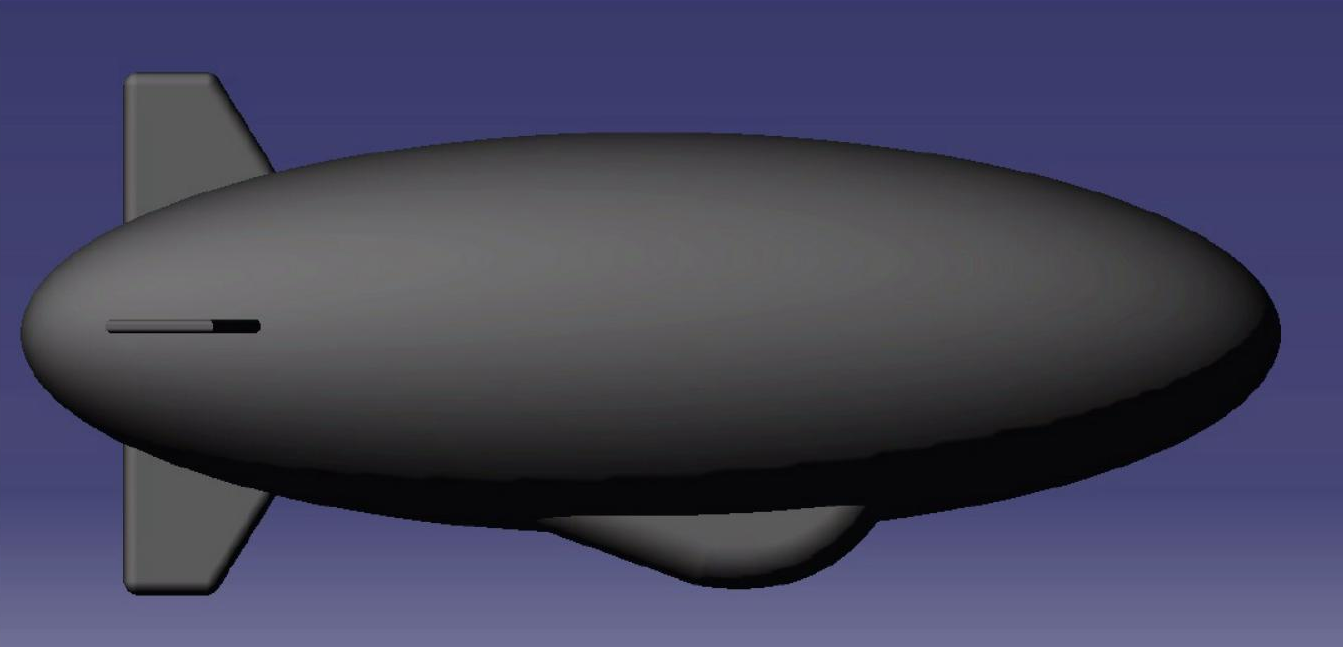
\includegraphics[scale=0.5]{figures/init.png}
\caption{Initial 3D sketch of the Airship}
\label{fig:init}
\end{figure}

As it is possible to see, this simplified view of the mechanical challenge, included the total development of the airship. The idea would be to include the solar panels on the top mounted on a wired mesh and the cargo bay attached in the bottom together with the propelling system.\\
Due to new developments in the project that included the introduction of an already built blimp (envelope), the focus of the mechanical design changed. The blimp to be used would be the TIF - 250 (Tethered Aerostats), Fig. \ref{fig:blimp}. This blimp has the capacity to lift a payload of about 2.5 Kg, it has a length of approximately 5 m and a diameter (in the center) of about 1.9 m.

\begin{figure}[bht]
\centering
\includegraphics[width=\textwidth]{figures/blimp-small.jpg}
\caption{TIF - 250 Blimp}
\label{fig:blimp}
\end{figure}

This blimp could serve the purpose of the U-SPACE project, its use would allow to focus only on the construction of the support for the power system, the cargo bay to accommodate the payload and also the integration of the propelling system. However, because it's a ready built blimp with a purpose different than the one intended, it is not as lightweight as it would might be needed. Nevertheless, an effort would be made to include light structures in the integration of all the other systems in this airship.

\subsection{Envelope}

As it was already stated, the blimp to be used is a ready built one. This blimp is normally used to accurately measure the wind direction, nevertheless it would had to fit the purpose of the U-SPACE project, due to the lack of time to build a new envelope. This way, the envelope is constituted by the blimp itself.  

\subsection{Cargo Bay}

The cargo bay is intended to accommodate both the payload and the electronics required to the purpose of the project. The main challenge in the construction of this cargo bay is the weight, it has to be lightweight but at the same time rigid enough to resist to some stress during the normal operation of the airship. To achieve this, balsa wood reinforced with carbon fibres was used, the box should be rigid enough to resist to the external forces, but lightweight enough to able a total maximum weight of all the structures of less than 1 Kg. Figures of the expected final cargo bay and of the current construction status are presented in Fig.\ref{fig:box} and \ref{fig:boxinit}, respectively. 

\begin{figure}[bht]
\centering
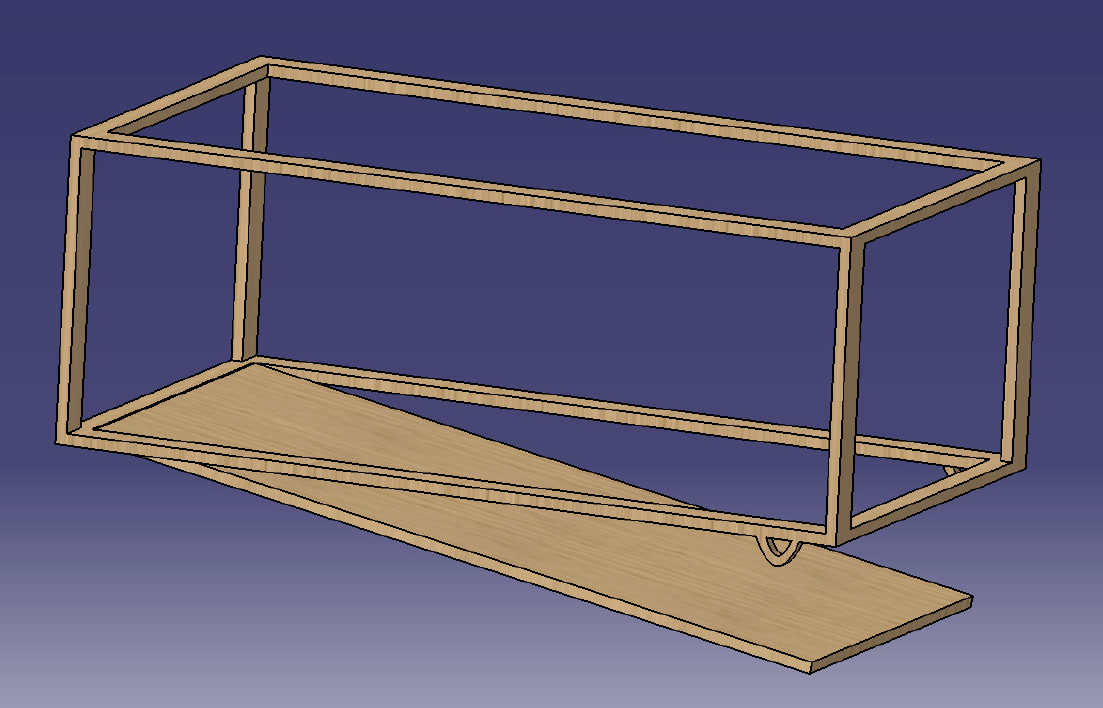
\includegraphics[scale=0.5]{figures/box.png}
\caption{Cargo Bay 3D sketch}
\label{fig:box}
\end{figure}

\begin{figure}[bht]
\centering
\includegraphics[width=\textwidth]{figures/boxinit-small.jpg}
\caption{Initial phase construction of the cargo bay}
\label{fig:boxinit}
\end{figure}

\subsection{Power System}

The biggest challenge of this project is to accommodate the power system having into account the maximum lift weight and also the power requirements that consequently influence the solar panels quantity and weight. Because different solar panels are still under test, it is still not decided how they will be mounted on the blimp. Nevertheless, the idea is to use a lightweight wired mesh that would serve as a support to the solar panels, attached to the wires with carbon fibre, and then this mesh would be consequently connected to blimp making use of 3 bands that would round the blimp distributing the weight along the envelope. This bands would be made of fibre glass reinforced rubber tape. \\
An idea of how the final product should look is presented in Fig. \ref{fig:mesh}.

\begin{figure}[bht]
\centering
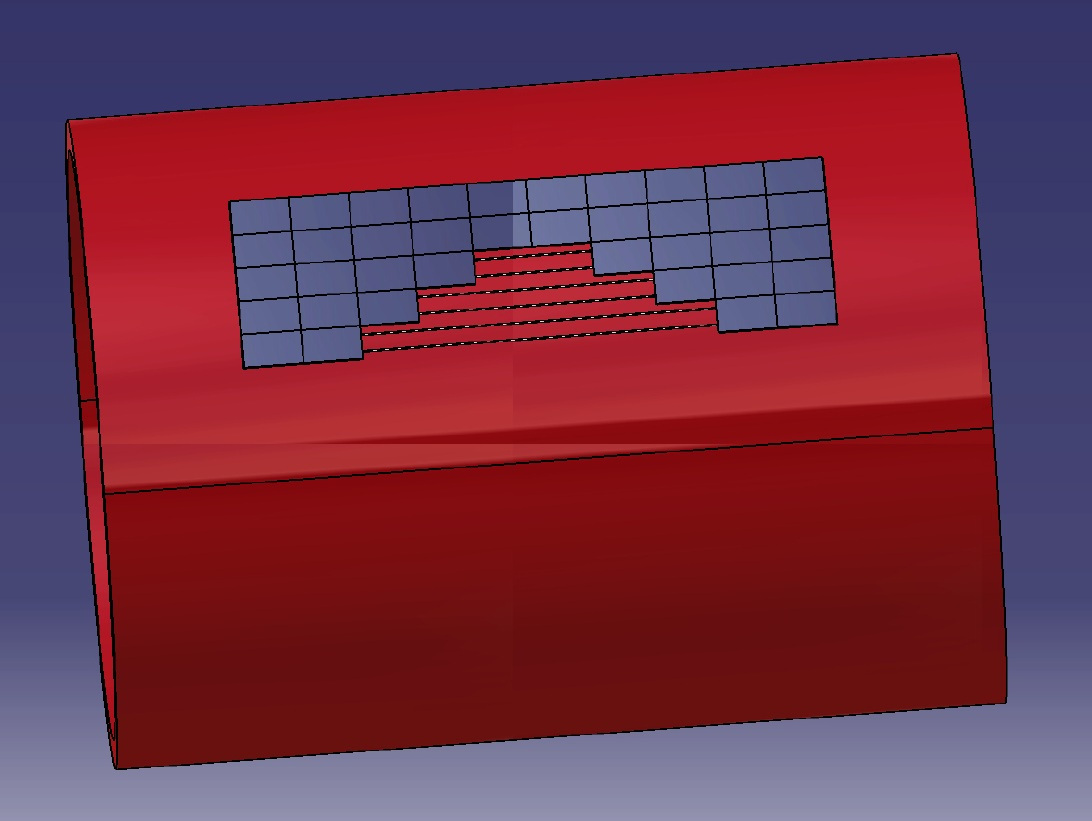
\includegraphics[scale=0.5]{figures/mesh.jpg}
\caption{Integration of the power system - 3D sketch}
\label{fig:mesh}
\end{figure}


\subsection{Propelling System}

The propelling system is to be integrated in a carbon fibre rod mounted on the top of the cargo bay. The 2 motors would be attached in the ends of the rod, outside the influence of the envelope and free to achieve their maximum aerodynamic capabilities. A hand sketch of this principle is showed in Fig.\ref{fig:prop}.

\begin{figure}[bht]
\centering
\includegraphics[width=\textwidth]{figures/prop-small.jpg}
\caption{Hand sketch of the integration of the propelling system}
\label{fig:prop}
\end{figure}

\section{Future Developments}

All the previously explained designs have to be built and tested. Conclusions have to be taken and inputs from the other systems have to be taken in consideration. Only after a careful building of the different structures to accommodate all the required systems, it will be possible to check if the requirement of the maximum lift weight - the most constrained one - is achieved. For now, the 3D designs, the intended to use materials and previous experiences in the field give hope that this constraint will be surpassed. \\
The following steps should be to finish the construction of the cargo bay, accommodate the propelling system into it and then proceed to the construction of the wiring mesh and consequent attachment of the solar panels.

\begin{scriptsize}
{\footnotesize •\begin{small}
{\normalsize •}
\end{small}}
\end{scriptsize}

%\section{Mechanical Interfaces}
%
%How does the MSE system interact with the other subsystems?
%
%\subsection{Mechanical Interface Control Drawing}
%
%Could not really find what this is and if we need it... Morten?
%
%\subsection{Accommodation Requirements}
%
%Same here...
%
%\section{Physical Properties}
%
%E.g. mass in launch configuration...
%
%\section{Structural and Mechanisms Analysis}
%
%This involves things like dynamic analysis and stress analysis, but as we didn't really do this, just briefly comment on it...
%
%\section{Mounting Attachments}
%
%Not sure what they mean with this... Attachment concept and foot pattern?
